Následující kapitola popisuje návrh nástroje pro administraci souborového systému ZFS. Zaměřuje se především na architekturu a bezpečnostní opatření navrhované aplikace.
\section{Požadavky}
Na začátku bychom měli stanovit funkcionalitu, která bude od aplikace vyžadována. Ještě jednou si připomeneme, že hlavním cílem této práce je vytvořit graficky orientovaný administrační nástroj pro správu souborového systému ZFS.

Souborový systém ZFS byl původně integrován do operačního systému Solaris. I~přes to, že dnes již existují operační systémy, na které bylo ZFS přeneseno, hlavní platformou aplikace bude právě operační systém Solaris.

Jelikož má nástroj být grafického charakteru, můžeme brát jako první požadavek na aplikaci přítomnost uživatelského rozhraní.

Jak bylo zmíněno v~úvodu, účelem toho nástroje má být ulehčení a zpřehlednění správy souborového systému ZFS a to i pro začínajícího administrátora. Bylo by tedy vhodné, aby zvolené uživatelské rozhraní bylo přehledné a jednoduché na používání.

ZFS je souborový systém určený především pro servery. Tyto počítače mohou být v~mnohých situacích pro administrátora fyzicky nedostupné. Abychom umožnili administrátorovi správu i v~těchto situacích, bude náš nástroj poskytovat možnost vzdáleného přístupu ke správě ZFS.

Na konci předchozí kapitoly jsme se dozvěděli, že většina nástrojů využívá takový způsob sběru dat, který uživateli v~některých situacích znemožňuje vidět přímo aktuální data. Tohoto problému bychom se při návrhu měli vyvarovat a zvolit takový způsob, který by uživateli zobrazil aktuální data při každém jeho požadavku.

Další nedostatek objevený při analýze již vytvořených nástrojů pro správu ZFS, je ten, že většina těchto nástrojů vůbec neposkytuje funkce pro administraci. Dovolují nám tedy daný souborový systém sledovat, ale ne ho spravovat. Jelikož je ZFS rozsáhlý souborový systém, obsahuje i velké množství funkcí a příkazů pro jeho správu. Bylo by tedy dobré některé základní funkce a příkazy pro administraci ZFS do tohoto nástroje zahrnout.

Posledním bodem požadavků by měla být bezpečnost. Hlavním důvodem proč se starat o~bezpečnost 0 je fakt, že pomocí ZFS lze jednoduchým příkazem zničit vše, co se na disku nachází. Jelikož se z~disku načítá při startu i operační systém, mohly by následky být fatální. Z~tohoto důvodu bude přístupná pouze specifikovaným uživatelům.

Pro shrnutí můžeme požadavky na administrační nástroj shrnout do následujících bodů:
\begin{itemize}
    \item Solaris
    \item Uživatelské rozhraní
    \item Jednoduchost a přehlednost
    \item Vzdálený přístup
    \item Aktuálnost dat
    \item Základní funkce pro administraci
    \item Bezpečnost
\end{itemize}

Pokud splníme všechny stanovené požadavky, můžeme uživateli zajistit bezpečnou správu souborového systému ZFS, která mu bude poskytovat aktuální informace.
\section{Možnosti uživatelských rozhraní}
Pro návrh uživatelského rozhraní aplikace přicházejí v~úvahu následující možnosti:
\begin{itemize}
  \item Příkazová řádka
  \item Grafické rozhraní
  \item Webové rozhraní
\end{itemize}
    \subsection{Příkazová řádka}
    Každý uživatel, který se někdy nějakým způsobem setkal s~administrací UNIXových operačních systémů, by měl mít alespoň nějaké povědomí o~tom, co je to příkazová řádka. Příkazová řádka je v~UNIXu nástroj, který umožňuje využívat různé příkazy. Je rychlý, nenáročný a jediné co potřebujete vědět je, jaký příkaz napsat a co daný příkaz udělá. Vše se obejde bez myši a klikání.

    Na druhou stranu může být pro začínajícího uživatele složité si všechny příkazy pamatovat a nějakou dobu trvá, než získá potřebné zkušenosti s~tímto nástrojem. Pokud uživatel příkazy příliš neovládá, je to pro něj spíše zpomalení práce než zrychlení.

    Protože jsme si v~požadavcích stanovili, že náš nástroj má být jednoduchý, přehledný a uživatelsky příjemný i pro začínající uživatele, je tato volba nevhodná.
    \subsection{Grafické rozhraní}
    Jelikož jsme zavrhli příkazovou řádku, je třeba přijít s~něčím, co bude pro uživatele přívětivé. Každý uživatel počítače se již jistě setkal s~pojmem grafické rozhraní. Pokud ne, pod pojmem grafické rozhraní si můžeme představit například některé programy z~operačního systému Windows. Prakticky všechno v~operačním systému Windows má svoje grafické rozhraní, aby měl uživatel přehled o~tom, co může v~daný okamžik využívat za funkce.

    Grafické rozhraní nám pomůže vyřešit problém s~uživatelským komfortem. Dále nám podle požadavků zbývá zvážit možnost vzdáleného přístupu. Ano i v~tomto případě bychom byli schopni tento požadavek splnit. Jde o~to, jak by to pro nás bylo pohodlné. Aplikace by musela být nainstalovaná na každém počítači, ze kterého bychom chtěli ZFS administrovat. Tento problém není nepřekonatelný, ale existuje ještě jedno komfortnější a dnes stále populárnější řešení.
    \subsection{Webové rozhraní}
    Nejkomfortnějším řešením je použití webového rozhraní. Hlavní výhodou toho řešení je fakt, že pro přístup k~aplikaci potřebujeme jen webový prohlížeč. Ten je dnes přítomný v~drtivé většině operačních systémů. Tato skutečnost nám přináší možnost přistupovat k~aplikaci z~webového prohlížeče v~libovolném operačním systému, přestože aplikace poběží na operačním systému Solaris.

    Webové stránky jsou navíc známé pro většinu uživatelů, a tak by při správném návrhu stránek neměl být sebemenší problém s~jednoduchostí a přehledností tohoto nástroje.

    Zbytek požadavků jako je bezpečnost jednoduše splníme pomocí správné implementace tohoto řešení.
\section{Architektura aplikace}
V~předchozí kapitole jsme pro náš nástroj zvolili možnost zobrazování dat pomocí webového rozhraní. Toto rozhraní se bude skládat z~webových stránek, které budeme chtít uživateli zobrazovat. Pro tento účel si budeme muset zvolit nebo implementovat nějaký webový server, který bude 0 komunikaci mezi naší aplikací a klientským prohlížečem. Jakmile uživatel požádá pomocí svého prohlížeče o~nějakou stránku, server tento požadavek obdrží a předá ho naší aplikaci. Aplikace ho vyhodnotí a prostřednictvím webového serveru pošle uživateli odpovídající odpověď.

Náš nástroj má sloužit pro správu souborového systému ZFS a tak bude nutné vymyslet, jak bude naše aplikace s~tímto systémem komunikovat. Administrátor může ZFS spravovat pomocí příkazů, které jednoduše zadá do příkazové řádky. Bude tedy nutné vymyslet vrstvu aplikace, která bude tyto příkazy sestavovat a následně provádět. Na obrázku \ref{architecture} můžeme vidět graficky znázorněnou komunikaci mezi hlavními komponenty aplikace.
\begin{figure}[h]
        \centering
        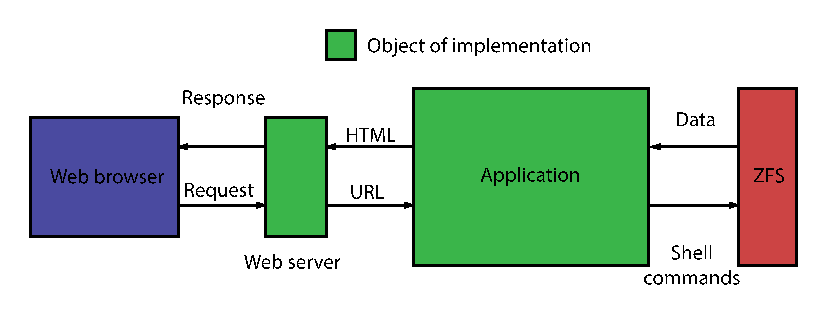
\includegraphics[scale=0.8]{appstructure.pdf}
        \caption{Struktura aplikace}
        \label{architecture}
\end{figure}
    \subsection{Architektura MVC}
    Nyní navrhneme řešení, jak bude aplikace fungovat uvnitř. Jak již bylo zmíněno, náš nástroj bude umožňovat správu souborového systému ZFS pomocí jeho základních funkcí. Tudíž ne všechny funkce budou ve výsledné implementaci zahrnuty. Z~tohoto důvodu je aplikaci nutno navrhnout tak, aby se dala jednoduše rozšiřovat o~potřebnou funkcionalitu.

    K~tomuto účelu použijeme objektový návrh společně s~architekturou MVC. Model-view-controller (MVC) je softwarová architektura, která rozděluje aplikaci do tří vrstev tak, že jsou na sobě minimálně závislé \cite{mvc}. Pokud bychom chtěli naši aplikaci rozšířit o~novou 0, jednoduše stačí rozšířit požadovanou vrstvu.

    Komponenty jednotlivých vrstev aplikace rozdělujeme na \emph{model}, \emph{view} a \emph{controller}.

        \subsubsection{Datová vrstva}
        \verb|Model| je označení pro třídu, která je součástí datové vrstvy aplikace. Úkol této třídy, stejně jako i celé datové vrstvy, je manipulace a práce s~daty. Všechny datové struktury si ZFS spravuje sám a my k~nim nemáme přímý přístup. Naše datová vrstva a její třídy nám tedy budou zajišťovat vykonávání ZFS příkazů, které budou sestaveny na základě dat předaných z~logické vrstvy.
        \subsubsection{Prezentační vrstva}
        Další vrstvou aplikace je tzv. prezentační vrstva. Tato vrstva se skládá ze tříd nesoucích obecný název \verb|View|. Hlavním úkolem této vrstvy je vykreslování dat uživateli. V~našem případě aplikace poběží na počítači se souborovým systémem ZFS a uživatel se k~ní bude připojovat pomocí webového prohlížeče. Naše prezentační vrstva tedy nebude přímo vykreslovat uživatelské rozhraní, protože neví kam. Pro zachování nezávislosti jednotlivých vrstev, bude prezentační vrstva pouze generovat HTML kód stránky z~dat, které jí budou předány. Následně takto vygenerovanou stránku předá zpět do logické vrstvy, která zařídí odeslání stránky uživateli.
        \subsubsection{Logická vrstva}
        Poslední vrstvou aplikace je logická vrstva. Hlavním úkolem této vrstvy je řízení toku dat mezi datovou a prezentační vrstvou. V~okamžiku, kdy webový server obdrží nějaký požadavek od uživatele, aplikace vybere z~logické vrstvy třídu, která dokáže tento požadavek vyřídit. Tato třída, kterou obecně nazýváme \verb|Controller|, může požádat datovou vrstvu, aby provedla potřebné operace se souborovým systémem nebo od souborového systému získala potřebná data. Následně data převede do potřebného formátu a požádá prezentační vrstvu o~jejich vykreslení. V~našem případě vykreslená data opět převezme a odešle klientovi.

        Komunikace mezi jednotlivými vrstvami aplikace je znázorněna na obrázku \ref{mvc}. Na obrázku je také vidět způsob předávání dat mezi webovým serverem a aplikací.

    \begin{figure}
        \centering
        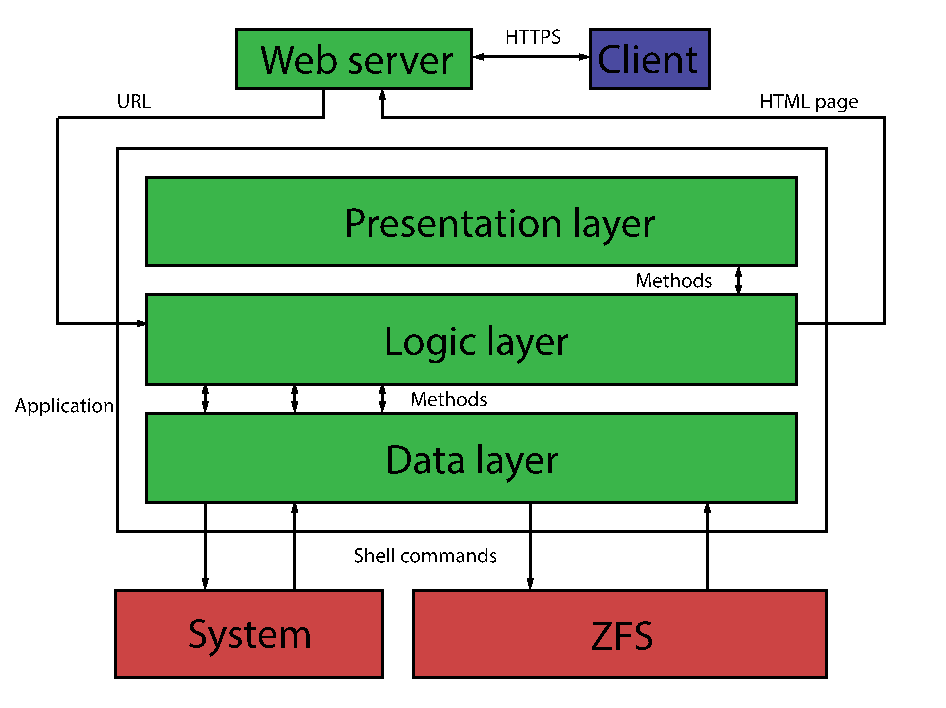
\includegraphics[scale=0.8]{mvc.pdf}
        \caption{Architektura aplikace}
        \label{mvc}
    \end{figure}
\section{Interakce s~aplikací}
K~aplikaci bude administrátor moci přistupovat pomocí webového prohlížeče. Tato výhoda pramení ze způsobu přenosu webových stránek pomocí protokolu HTTP, který je pro tento účel určený. Jeho definici můžeme najít v~RFC dokumentu \cite{RFC2616}. Tento protokol je postavený na architektuře klient-server, kdy klient posílá požadavky na webový server a ten klientovi odpovídá v~podobě HTML dokumentu. Jak již bylo zmíněno, výhodou tohoto způsobu je oddělenost serveru a klienta.

Uživatel bude pomocí webového prohlížeče vznášet požadavky na webový server v~podobě URL. Uniform resource locator (URL) se používá pro lokalizování zdrojů na internetu poskytnutím jedinečného řetězce znaků \cite{RFC3986}. HTTP požadavek, který uživatel bude pomocí webového prohlížeče odesílat, obsahuje právě tento URL řetězec. Tím administrátor specifikuje jakou stránku chce zobrazit popřípadě jakou akci chce povést.

Naši aplikaci tedy postavíme tak, aby byla schopná přijmout URL řetězec a na základě jeho struktury provedla určitou akci.

\section{Bezpečnost}
Další důležitou kapitolou v~procesu návrhu administrátorského nástroje je bezpečnost.

Některé příkazy poskytované souborovým systém ZFS jsou dostupné každému uživateli v~systému. Jedná se hlavně o~příkazy, které vypisují nejrůznější informace o~stavu souborových systémů a poolů. Prováděním těchto příkazů se v~nastavení ZFS nic nezmění, a proto nemůže dojít k~poškození nebo ztrátě dat. Na druhou stranu ZFS nabízí příkazy, které běžní uživatelé nemohou využívat. K~provádění těchto příkazů je potřeba oprávnění \emph{root} uživatele. Jedná se zejména o~příkazy, které vytvářejí, mění nebo ničí souborové systémy či pooly. Toto chování je naprosto pochopitelné, protože nesprávným nebo neuváženým použitím těchto příkazů může dojít ke zničení cenných dat nebo celého operačního sytému.

Našim cílem je vytvořit nástroj pro správu souborového systému ZFS. Je tedy zřejmé, že budeme potřebovat, aby naše aplikace dokázala využívat i příkazy, které nejsou běžným uživatelům dostupné. V~operačním systému Solaris, kde naše aplikace poběží, dostává každý spuštěný proces tzv. identitu. Tato identita spojuje běžící proces s~uživatelem, pod kterým byl proces spuštěn. Díky tomu je operační systém schopen určit, jaká práva proces má a co vše může v~systému využívat. Pokud bychom spustili naší aplikaci pod uživatelem, který nemá právo využívat některé příkazy souborového systému ZFS, pak by je nemohl využívat ani náš nástroj. Tento fakt nás tedy vede k~tomu, abychom naší aplikaci spouštěli pod uživatelem, který má právo vykonávat všechny ZFS příkazy.

Máme tedy aplikaci, která může v~systému provádět potřebné příkazy a je dostupná na nějaké URL adrese. Problém přístupu neoprávněných uživatelů k~nebezpečným příkazům byl vyřešen na úrovni systému a jednoduše nemohli nebezpečné příkazy spouštět. Nyní jsme aplikaci pustili pod uživatelem, který tato práva vlastní a navíc má tato aplikace veřejné webové rozhraní, které je dostupné na stanové URL adrese. Každý kdo tuto adresu zná, může v~tuto chvíli pomocí webového prohlížeče k~aplikaci přistoupit a provádět jejím prostřednictvím nebezpečné příkazy. To není úplně ideální případ. My bychom chtěli, aby k~aplikaci mohli přistupovat jenom oprávnění uživatelé pomocí přihlašovacího jména a hesla. K~tomuto použijeme vlastnost HTTP protokolu Basic Authentication, která nám zajistí přístup jen pro autentizované uživatele.

Aplikace bude přístupná jen pro oprávněné uživatele, kteří se autentizují pomocí metody Basic 0. To s~sebou přináší další starosti, protože uživatelské jméno a heslo musíme ověřit. Tyto citlivé informace pomocí HTTP protokolu putují přes počítačovou síť až ke koncovému webovému serveru. Podle specifikace \cite{RFC2616} HTTP protokol neumožňuje šifrování. To znamená, že potencionální útočník může na síti odposlechnout požadavek, který obsahuje uživatelské jméno a heslo a použít tyto údaje pro vstup do aplikace. Z~tohoto důvodu budeme přenos dat šifrovat pomocí HTTPS protokolu.
    \subsection{Systémový uživatel}
    \label{sysuser}
    Z~důvodů uvedených výše budeme potřebovat vhodného uživatele, pod kterým budeme tuto aplikaci spouštět. V~úvahu přicházejí následující možnosti:
    \begin{itemize}
      \item uživatel \emph{root}
      \item role (RBAC)
    \end{itemize}

    První možností je zvolit uživatele \emph{root}. Tento uživatel má právo na všechny operace v~systému. Tato volba by sice náš problém vyřešila, ale přinesla by další bezpečnostní rizika. Pokud bychom spustili aplikaci s~identitou uživatele \emph{root}, pak by tato aplikace mohla v~systému provádět všechny příkazy. To by bylo pro naši aplikaci zbytečné. Nám bude stačit, pokud aplikace bude moci využívat přesně ty nástroje, které ke své správné funkčnosti potřebuje. Dalším rizikem je fakt, že by potenciální útočník mohl tato práva nějakým způsobem zneužít.

    Druhá možnost, která přichází v~úvahu, je použití tzv. RBAC. Jedná se o~rozšíření bezpečnostního modelu, které nám umožňuje kontrolovat přístup uživatelů k~úkonům přístupným pouze pro superuživatele \emph{root}. V~nerozšířeném bezpečnostním modelu jste buď uživatelem s~omezenými možnosti a nebo jste superuživatel a můžete všechno \cite{RBAC}. Ve zkratce RBAC umožňuje vytváření tzv. rolí, které se chovají téměř jako normální uživatel. Rozdíl je v~tom, že na roli se nedá přihlásit přímo. Do systému se nejprve musí přihlásit klasický uživatel, který si poté smí přiřadit určité role. Rolím jsou přiřazovány bezpečnostní profily, které obsahují jednotlivá privilegia.

    Pro bezpečnost našeho nástroje si tedy vytvoříme roli, které přiřadíme potřebná oprávnění pro vykonávání následujících příkazů:
    \begin{itemize}
      \item \emph{zfs}
      \item \emph{zpool}
      \item \emph{format}
      \item \emph{fdisk}
    \end{itemize}

    Aplikaci budeme spouštět pod touto rolí. Ve výsledku aplikace bude mít veškerá oprávnění pro svoji správnou činnost a bezpečnostní rizika budou minimální.
    \subsection{HTTP Basic Authentication}
    \label{httpauth}
    Basic 0 je způsob autentizace uživatelů pomocí protokolu HTTP. Pokud webový server vyžaduje tuto metodu ověření, uživatel je před přístupem k~obsahu vyžádán o~autentizaci pomocí jména a hesla. Jméno a heslo je pak spolu s~požadavek odesláno webovému server k~ověření \cite{RFC2617}.

    Pro naší aplikaci to znamená, že webový server bude muset umět ověřit uživatele oproti lokální databázi. Pokud se uživatelské jméno a heslo odeslané webovým prohlížečem bude shodovat s~uživatelskými údaji v~lokální databázi, bude uživateli umožněn vstup do aplikace. Do všech částí aplikace bude umožněn vstup pouze autentizovaným uživatelům.

    \subsection{HTTPS}
    \label{https}
    HTTP protokol nám neumožňuje nijak šifrovat data, která jsou přenášena. Jelikož jsou po síti přenášena citlivá data jako je uživatelské jméno a heslo, musíme zajistit šifrování tohoto přenosu. HTTPS je protokol, který nám to umožní. Tento protokol ve svém základu využívá ke komunikaci HTTP protokol, ale rozdíl je v~tom, že přenášená data jsou šifrována pomocí SSL nebo TSL \cite{RFC2818}.

    Použití protokolu HTTPS zajistí naší aplikaci, že bude pro útočníka téměř nemožné získat uživatelské údaje, které byli použity pro vstup do aplikace.
    \subsection{Shrnutí}
    Pro shrnutí zopakujeme, jaké bezpečnostní opatření budou provedena pro zajištění aplikace. Vytvoříme systémovou roli pomocí RBAC, která bude mít privilegia k~vykonávání potřebných operací. Výsledná aplikace bude spouštěna pod touto rolí. K~autentizaci uživatelů, kteří budou přistupovat k~aplikaci, použijeme metodu Basic protokolu HTTP. Uživatele budeme ověřovat proti lokální databázi uživatelů. A~konečně celý přenos dat mezi webovým serverem a klientem zašifrujeme pomocí protokolu HTTPS.

\section{Integrace do systému}
Pro ulehčení správy celé aplikace ji zaregistrujeme v~operačním systému Solaris jako službu. Docílíme tím toho, že se operační systém bude sám starat o~zapínání, vypínání a restartování celé aplikace. Samozřejmě, že budeme stále schopni explicitně říci, jestli se má daná aplikace spouštět.

Service Management Facility je v~operačním systému Solaris nástroj pro spravování služeb. Nahrazuje tím tradiční způsob spravování služeb pomocí \emph{init} skriptů, který byl běžný v~dřívějších verzí operačního systému Solaris a ostatních UNIXových operačních systémech. Velkou výhodou SMF je možnost definování závislostí dané služby na ostatní službách. Tím dokážeme stanovit, že se daná služba nespustí, dokud nebudou spuštěny všechny služby stanovené v~závislostech. SMF také uchovává veškeré informace o~startu, běhu i ukončování služby v~logu. Administrátor má tedy kdykoli možnost tyto logy prozkoumat a získat požadované informace. V~pozadí každé služby zaregistrované v~SMF je tzv. manifest \cite{SMF}.
    \subsection{Manifest}
    Manifest je XML dokument, který danou službu popisuje. Právě zde administrátor stanovuje, na kterých službách bude tato služba závislá nebo jak se daná služba jmenuje. V~našem případě to znamená, že si budeme muset tento manifest vytvořit a zaregistrovat službu v~SMF.
    \subsection{Metody}
    Důležitou součástí manifestu jsou metody, které SMF říkají, jak má danou službu zapnout nebo vypnout. V~těchto metodách se může spouštět více procesů, které jsou svázány dohromady jako součást dané služby. Administrátor se pak stará jenom o~službu jako takovou a nemusí vůbec vědět, jaké procesy byly v~rámci služby spuštěny \cite{SMF}. Mimo jiné můžeme v~manifestu určit tzv. kontext metod. Tato vlastnost nám dovoluje určit pod jakým uživatelem mají být jednotlivé metody vykonávány. V~kontextu naší aplikace to znamená, že metody služby budou spouštěny pod námi vytvořenou rolí, která bude mít dostatečná práva.
    \subsection{Shrnutí}
    Zaregistrování aplikace jako služby v~operačním systému Solaris nám přinese následující výhody pro správu této aplikace. Administrátor bude mít jasný přehled nad tím, zda je daná služba spuštěna. Dále bude moci jednoduše danou službu spustit popřípadě zastavit. Pokud dojde k~nějakému problému při spuštění dané služby, SMF administrátorovi poskytne informace o~zdroji tohoto problému. V~poslední řadě SMF také umožní automatické spuštění služby při startu systému.

    Jako pracovní název aplikace zvolíme \emph{wzfsadm}, který vznikl spojením slov web, ZFS a administrace. Z~názvu je jasně patrné, že nástroj bude sloužit pro webovou administraci souborového systému ZFS.


